\documentclass[10pt, a4paper]{article}
\usepackage[french]{babel}
\usepackage[utf8]{inputenc}

\usepackage{geometry}
\geometry{lmargin=2cm, rmargin=2cm, vmargin=2cm} %%% Marges

\usepackage{listings}
\lstset{language=XML,basicstyle=\footnotesize\ttfamily}

\usepackage{amsmath, amssymb}
\usepackage{graphicx,xspace,color,hyperref}
%\usepackage{enumerate}
\usepackage{multicol}

\author{}
\title{}
\date{\today}

%%%%%%%%%%%%%%%%%%%%%%%%%%%%%%%%%%%%%%%%%%%%%%%%%%%%%%%%%%%%%%%%%%%%%%%%
\begin{document}

\renewcommand{\labelitemi}{\textbullet}  %%% Puce enumerations

\renewcommand{\leq}{\leqslant}              %%% <= plus propre
\renewcommand{\geq}{\geqslant}              %%% >= plus propre

%%%%%%%%%%%%% D E B U T %%%%%%%%%%%%%%%

\begin{center}\Huge
\textbf{SVG + Droste effect = VINS !}
\end{center}

\section{Introduction}

SVG (\emph{Scalable Vector Graphic}) est un langage de balisage (\emph{markup language}) au format XML
permettant de décrire des \emph{images vectorielles}.

Contrairement
aux images matricielles (\emph{raster} ou \emph{bitmap}, formats BMP,
GIF, JPEG, PNG, \textit{etc}), qui ont une
taille bien définie et sont décrites par la donnée de la couleur de
chacun des pixels, les images vectorielles (formats PDF, PS, SVG) sont décrites par la
donnée des formes géométriques élémentaires (lignes, rectangles,
cercles, \textit{etc}) qui les composent et n'ont pas de taille fixe.

L'intérêt
des images vectorielles est le passage à l'échelle : tandis qu'il
n'est pas possible d'agrandir une image matricielle sans faire
apparaître tôt ou tard les pixels qui la composent, une image
vectorielle peut être affinée à l'infini, à la taille et la résolution
que l'on souhaite. Il est par exemple possible de zoomer à l'infini
sur les caractères d'un document PDF ou PostScript : à chaque zoom,
la portion affichée de la page sera recalculée par le lecteur avec une
résolution de plus en plus grande pour que l'image apparaisse nette.

Les formats vectoriels sont inadaptés à la description d'images
photographiques (qui se décomposent très mal en un assemblage de formes
géométriques élémentaires) mais très performants pour des assemblages
géométriques complexes. Le jeu vidéo \emph{Another World} (1991), utilisant
un moteur intégralement vectoriel, ce qui était inédit à l'époque, est
une belle illustration de cette performance (le format vectoriel
permettant de décrire des scènes graphiquement très riches de façon
très compacte en mémoire).

Un écran d'ordinateur n'étant qu'une matrice de pixels, l'affichage
d'une image vectorielle passe par sa conversion en image matricielle
d'une taille donnée, arbitrairement grande. Ce processus est appelé \emph{rasterisation}.

L'objectif de ce projet est d'implémenter la rasterisation d'une
variante originale, appelée VINS, du format SVG.

\section{Le format SVG}

\noindent Voici un exemple simple de document SVG et l'image correspondante.

\begin{multicols}{2}
\lstinputlisting{ex0.svg}

\hspace{4cm}
\includegraphics[width=2cm]{ex0.png}
\end{multicols}

Une spécification complète, normalisée par le W3C, de SVG peut être
trouvée ici : \url{http://www.w3.org/TR/SVG/}. Dans la suite, nous ne
travaillerons qu'avec quelques balises simples, on pourra donc se
contenter de parcourir la section \emph{Shapes} du tutoriel du W3C : \url{http://www.w3schools.com/svg/}.

\section{Le format VINS}

\noindent Le format VINS (\emph{VINS Is Not SVG}) reprendra un sous ensemble
minimaliste des balises du langage SVG :
\begin{itemize}
\item \texttt{<line x1="$x_1$" y1="$y_1$" x2="$x_2$" y2="$y_2$" />}
\item \texttt{<rect x="$x$" y="$y$" width="$w$" height="$h$" />}
\item \texttt{<polygon points="$x_1$,$y_1$ $x_2$,$y_2$ $\ldots$ $x_n$,$y_n$" />}
\item \texttt{<circle cx="$x$" cy="$y$" r="$r$" />}
\end{itemize}
où toutes les dimensions ($x$, $y$, $w$, \textit{etc}) sont des nombres
flottants positifs.

Un document SVG n'étant qu'une liste finie de telles primitives, une
limitation importante est qu'il ne permet pas de décrire des objets
réellement infinis\ldots{} Afin de palier ce défaut, le format VINS introduit
une unique balise supplémentaire :
\begin{center}
\texttt{<call target="{\it cible}" x="$x$" y="$y$" width="$w$" height="$h$" />}
\end{center}
où \textit{cible} vaut soit le nom d'un fichier VINS externe,
soit \texttt{self} pour désigner le fichier courant, et la balise
\texttt{call} a pour effet de faire référence à l'image décrite par le fichier
cible dans le rectangle défini par les attributs \texttt{x}, \texttt{y}, \texttt{width} et \texttt{height}.

Un document VINS complet ne sera qu'une séquence finie de balises
parmi les cinq précédentes, précédée par une balise de début
\texttt{<vins width="$w$" height="$h$">} et terminée par une balise de
fin \texttt{</vins>}. Les attributs \texttt{width} et \texttt{height}
de la balise \texttt{vins} ne définissent \textbf{pas} la taille (en pixels) de
l'image vectorielle (par définition, celle-ci n'en a pas) mais les
dimensions de la zone de dessin (c'est-à-dire les valeurs maximales des coordonnées flottantes des points manipulés).

On trouvera ci-après quelques exemples simples.

\begin{multicols}{2}
\lstinputlisting{zigzag.vins}

\hspace{3cm}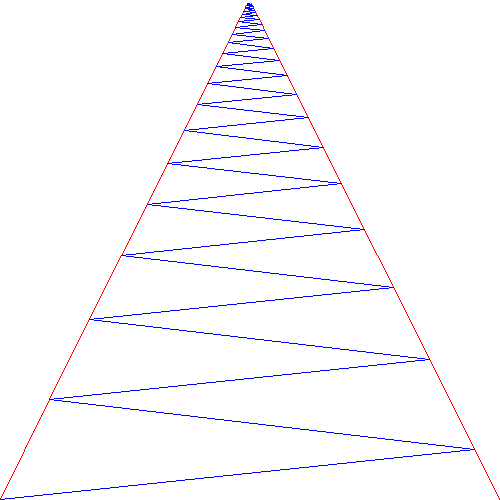
\includegraphics[width=4cm]{zigzag.png}
\end{multicols}

\begin{multicols}{2}
\lstinputlisting{sierp.vins}

\hspace{3cm}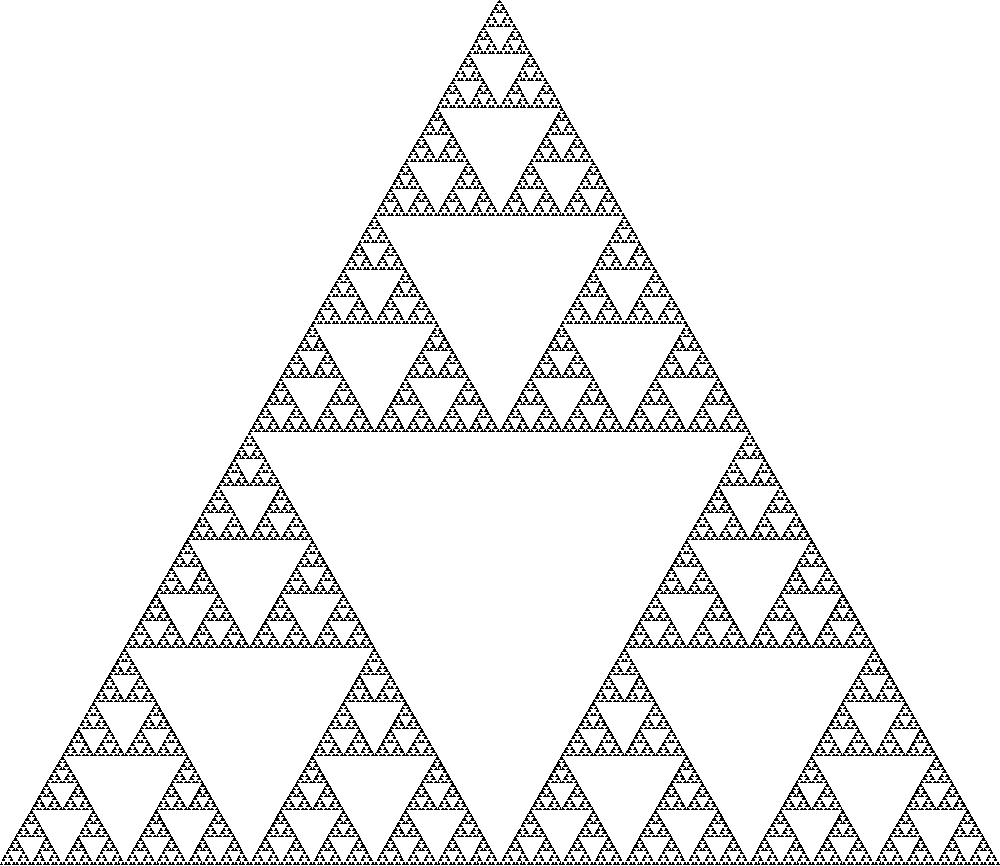
\includegraphics[width=4cm]{sierp.png}
\end{multicols}

\begin{multicols}{2}
\lstinputlisting{bisierp0.vins}
%\lstinputlisting{bisierp1.vins}

\vspace{4cm}\hspace{3cm}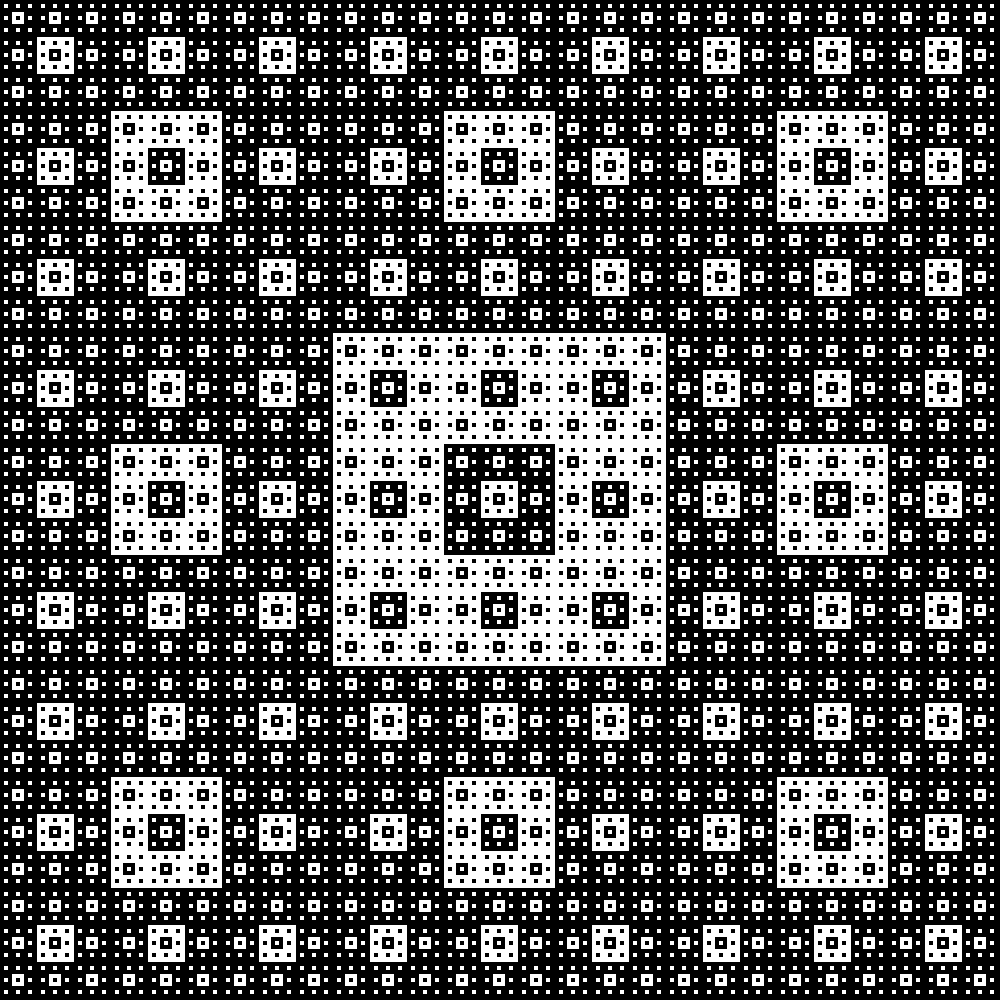
\includegraphics[width=4cm]{bisierp.png}
\end{multicols}

\section{À vous de jouer\ldots}

Vous devez écrire en Java un programme \texttt{vins2png} qui produit une image PNG obtenue par rasterisation à une résolution arbitrairement grande d'un fichier VINS. Ainsi, l'exécution de \texttt{./vins2png in.vins 1000 1000 out.png} devra produire une image PNG \texttt{out.png} de taille $1000\times1000$ pixels à partir de l'image VINS \texttt{in.vins}.

Afin de parser le XML d'un fichier VINS, vous pourrez utiliser les bibliothèques \texttt{javax.xml.parsers} et \texttt{org.w3c.dom} afin de récupérer une représentation facile à manipuler et conforme au modèle objet DOM (\url{http://www.w3schools.com/dom/}) du W3C.

Évidemment, on ne vous demande ni de manipuler directement le format PNG, ni d'implémenter par vous même les primitives de dessin. Vous utiliserez pour cela les bibliothèques \texttt{java.awt} (pour les primitives permettant de dessiner des lignes, des cercles, \textit{etc}) et \texttt{javax.imageio} (pour enregistrer au format PNG).

\section{Compléments possibles}

Prendre en charge plus de balises de dessin de SVG ; gérer une partie des styles et couleurs de SVG ; gérer les rotations via un attribut \texttt{angle} ajouté à la balise \texttt{call} ; gérer au mieux les imprécisions du calcul ; optimiser la gestion des appels récursifs de paramètres identiques (mêmes cible et dimensions) redondants ; proposer une interface graphique avec outil de zoom pour jouer avec l'image en temps réel\ldots

%%%%%%%  F  I  N  %%%%%%%%%%%%%%%
\end{document}
